\section{Experiment and Discussion}

% \KZ{Main content (the tables) can't go into the fifth page, or the paper will be
% rejected without review.}

% \noindent\textbf{Implementation Details}~~For base generation model, we fine-tuned GPT2~\citep{gpt2}
% and BART-base~\citep{bart} on $\alpha$\textit{NLG}. For teacher model in EBM, we fine-tuned BERT-base~\citep{bert}
% and RoBERTa-base~\citep{roberta} on $\alpha$\textit{NLI}.\JQ{repeat with the "section 2 initial model training"} The tolerant value $\tau$ for EBM training is set
% to $1e-3$. In the KL-Adaptive DPG algorithm, we set $K = 20480$ for the estimation of $\hat{Z}_i$ and $D_{KL}$.
% The maximum training step is set to $512$k. The beam search size $k_{bs}$ is $4$.
% \KZ{Difference between EBM(GPT2) and GPT2 is not big, same goes with BART. This seems to suggest
% that the EBM is not that useful.}

\noindent\textbf{Automatic Evaluation}~~We use BLEU~\citep{bleu}, ROUGE-L~\citep{lin-2004-rouge}, METEOR~\citep{banerjee-lavie-2005-meteor} and CIDEr~\citep{cider} 
for automatic evluation. 
Besides of the above metrics, we also evaluate the $\mathcal{ART}$ \textit{score} of the generation texts,
which should be a natural and coherent evaluation metric but is ignored in previous work.
We use the top-tier models on the $\alpha$\textit{NLI} leaderboard\footnote{https://leaderboard.allenai.org/anli/submissions/public}
to score the generated texts. Since we have used RoBERTa as teacher model in the EBM, we use two more strong
$\alpha$\textit{NLI} model as scorer for fair comparison.
One is DeBERTa~\citep{deberta}, a recently published large pre-trained language model reaching to top-1 on
varied of benchmarks. Another one is $L2R^2$~\citep{l2r2}, which solved $\alpha$\textit{NLI}
by leveraging ranking loss.% and reaching the 3rd place on the leaderboard.
\begin{table*}[ht]
\centering
\small
\begin{tabular}{lccccccc}
%\hline
\toprule
\multirow{2}{*}{} & \multirow{2}{*}{BLEU-4} & \multirow{2}{*}{ROUGE-L} & \multirow{2}{*}{METEOR} & \multirow{2}{*}{CIDEr} & \multicolumn{3}{c}{$\mathcal{ART}$ \textit{score}} \\ \cline{6-8}
 &  &  &  &  & RoBERTa & $L2R^2$ & DeBERTa \\ \midrule
GPT2-fixed$^{\dagger}$ & 2.23 & 22.83 & 16.71 & 33.54 & 42.32 & 40.19 & 41.38 \\
GPT2+COMeT txt$^{\dagger}$ & 2.29 & 22.51 & 16.73 & 31.99 & 48.22 & 42.56 & 48.53 \\
GPT2+COMeT emb$^{\dagger}$ & 3.03 & 22.93 & 17.66 & 32.00 & 49.34 & 42.64 & 49.64 \\
GRF~\citep{grf} & {\ul 11.62} & 34.62 & 27.76 & 63.76 & 66.89 & 55.76 & 65.79 \\ \midrule
GPT2-FT$^{\ddagger}$ & 8.49 & 31.09 & 22.87 & 54.10 & 49.32 & 53.34 & 49.54 \\ 
EBM(GPT2+BERT) & 8.59 & 31.27 & 23.43 & 54.80 & 50.46 & 53.45 & 51.70 \\
EBM(GPT2+RoBERTa) & 8.86 & 31.63 & 23.95 & 55.25 & 55.39 & 54.06 & 54.77 \\
BART-FT$^{\ddagger}$ & \textbf{11.79} & 35.57 & \textbf{28.09} & \textbf{67.33} & 66.12 & {\ul 57.53} & 64.98 \\
EBM(BART+BERT) & 11.60 & \textbf{35.62} & 27.93 & {\ul 66.80} & {\ul 66.39} & 57.50 & {\ul 65.84} \\
EBM(BART+RoBERTa) & 11.54 & {\ul 35.58} & {\ul 28.00} & 66.69 & \textbf{70.01} & \textbf{57.77} & \textbf{67.08} \\ \midrule
Human$^\diamondsuit$ & - & - & - & - & 77.31 & 64.04 & 79.80 \\ \bottomrule
\end{tabular}
\caption{
    $\dagger$: Baseline Models and results from ~\citet{Bhagavatula2020Abductive}. 
    $\diamondsuit$: We feed reference hypothesis to $\phi(x)$ to obtain human performance as upper bound.
    $\ddagger$: The base generation model we fine-tuned on $\alpha$\textit{NLG}.
    \textbf{Bold face}: highest score. {\ul Underline}: second highest score.
}
\label{exp-result}
\end{table*}

We show the experiment results on the $\alpha$\textit{NLG}
test set in Table~\ref{exp-result}. We observe that compared with the initial
generation model GPT2 and BART-base, our proposed EBM model has improved the $\mathcal{ART}$ \textit{score}
across all of the scorers, demonstrating the effectiveness of our methods.
In particular, the improvement of using RoBERTa as teacher model in EBM
more significant than using BERT. % \JQ{by ... with which model. add some details}
Compared with GRF~\citep{grf}, EBM(BART+RoBERTa) obtains a comparable score on the traditional automatic evluation metrics, but outperforms
it on $\mathcal{ART}$ \textit{score} by $3.28$. 
% In theory, our EBM setting is orthogonal to their methods and we leave
% further combination for future work.

\noindent\textbf{Learninng Curves}~~We plot the learning curve in Figure~\ref{fig:learning_curve}.We evaluate 
$\pi_\theta$ on the validation set and compute the corresponding $\mathcal{ART}$ \textit{score} $\phi(x)$.
We find that the $\mathcal{ART}$ \textit{score} of both GPT2-based and BART-based EBM increase stably during training, demonstrating the effectiveness and feasibility of posing the consistency and coherency of generated hypothesis to
training objective. 
With the same RoBERTa as the $\phi(x)$ scorer model, we find that BART-based geneartion model significantly 
outperformed GPT2-based. 
% One possible reason is that the BERT-based encoder in BART can better capture the underlying context in $\alpha$\textit{NLG}. 
One possible reason is that BART has a BERT-based encoder, which can capture and encoder the
underlying context bidirectionally for abudtive reasoning while GPT2 cannot. 
% \JQ{This explanation is not clear, show the key difference of GPT2 and BERT that helps with the context understanding .}

\noindent\textbf{Effect of The Teacher Model}~~In our methods, we expect the teacher model can give a reasonable
and precise score to evaluate how well the generated text fit into the context. Hence the performance of the
teacher model should be a critical point in our methods. From Table~\ref{exp-result} we can find that a RoBERTa EBM
is better than a BERT-based EBM. We fine-tuned RoBERTa on less training data of
$\alpha$\textit{NLI} and report the improvement of $\mathcal{ART}$ \textit{score} against the base generation
model($\ddagger$) in Table~\ref{exp-result}. From Table~\ref{data-ratio-test} we can see that the improvements 
of $\mathcal{ART}$ \textit{score} and the accuracy on $\alpha$\textit{NLI}
dev set are positively related, which demonstrates that a better-trained $\alpha$\textit{NLI} model can bring more improvement.
\begin{figure}[t]
    \centering
    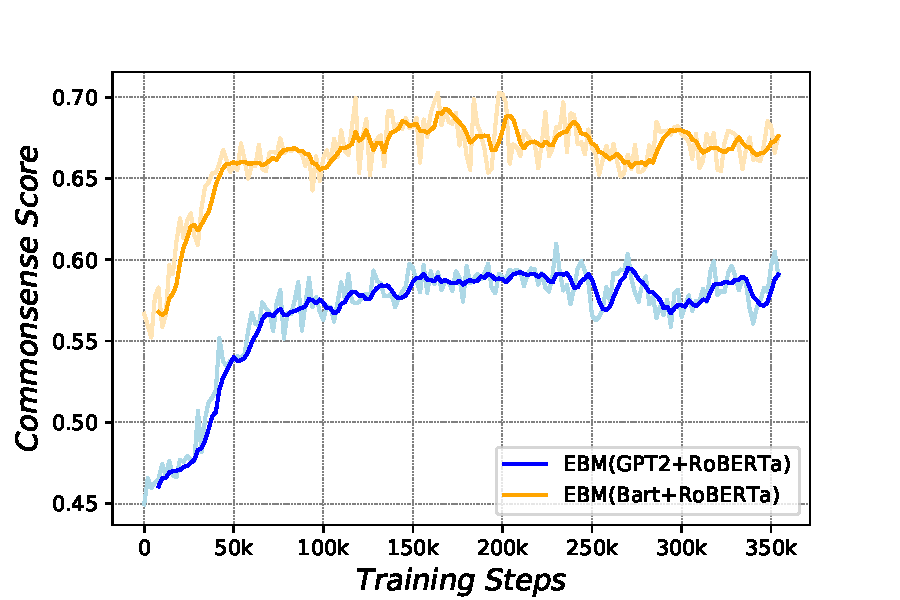
\includegraphics[width=1.0\columnwidth]{figs/learning_curve.pdf}
    \caption{Learning curve for the EBM on $\alpha$\textit{NLG}. 
    %The trend is highlighted for better visualization.
    }
    \label{fig:learning_curve}
\end{figure}
\begin{table}[ht]
\small
\centering
\begin{tabular}{lccc}
\toprule
Ratio of data & \multicolumn{1}{l}{GPT2} & \multicolumn{1}{l}{BART} & \multicolumn{1}{l}{$\alpha$\textit{NLI} dev acc} \\ \midrule
20\% & +1.76 & +1.12 & 68.05 \\
40\% & +2.20 & +1.43 & 70.28 \\
60\% & +2.77 & +2.02 & 72.43 \\
80\% & +4.55 & +2.57 & 73.56 \\
100\% & +6.07 & +3.89 & 74.98 \\ \toprule
\end{tabular}
\caption{Improvement of $\mathcal{ART}$ \textit{score} w.r.t. RoBERTa trained on different ratio of $\alpha$\textit{NLI} as teacher model.}
\label{data-ratio-test}
\end{table}
\begin{table}[ht]
\small
\centering
\begin{tabular}{lcc|cc}
\toprule
 & \multicolumn{2}{c|}{\begin{tabular}[c]{@{}c@{}}EBM\\ (GPT2+RoBERTa)\end{tabular}} & \multicolumn{2}{c}{\begin{tabular}[c]{@{}c@{}}EBM\\ (BART+RoBERTa)\end{tabular}} \\ \midrule
\multicolumn{1}{l|}{} & vs GPT2-FT & vs GRF & vs BART-FT & vs GRF \\
\multicolumn{1}{l|}{W} & 0.163 & 0.236 & 0.203 & 0.310 \\
\multicolumn{1}{l|}{T} & 0.753 & 0.490 & 0.665 & 0.460 \\
\multicolumn{1}{l|}{L} & 0.083 & 0.277 & 0.132 & 0.230 \\ \hline
\multicolumn{1}{l|}{$\kappa^{\dagger}$} & 0.634 & 0.602 & 0.628 & 0.594 \\ \toprule
\end{tabular}
\caption{Percentage of win(\textbf{W}), tie(\textbf{T}) and lose(\textbf{L}). $\dagger$: Fleiss' Kappa for annotator agreement.}
\label{humaneva}
\end{table}
\KZ{My suspect is that as you increase the aNLG training data you get
a similar curve up. So the conclusion may be that adding aNLI data
is the same as adding aNLG data. That will nullify the contribution of
this approach. You need to show otherwise.}

\noindent\textbf{Human Evaluation}~~We randomly sample 100 inputs from test set to investigate the reliability
of the $\mathcal{ART}$ \textit{scores}. Specifically, we ask $3$ annotators to make a preference
among \textit{win}, \textit{lose} and \textit{tie} given the input observations and two outputs
by our model and a baseline respectively, according to the criteria that whether the output sentence
explains well the observations. Results are shown in Table~\ref{humaneva}. We can see that the EBM(GPT2+RoBERTa)
obtains more \textit{win} than GPT2-FT but less than GRF, while EBM(BART+RoBERTa) obtains more \textit{win}
than both baselines, which is consistent with the results in Table~\ref{exp-result} and thus supports the
reliability of $\mathcal{ART}$ \textit{score}.
